\chapter{Games deployment and evaluation}
\label{ch:gamesDepl}
We deployed the games presented in chapter 3 in teams working on Intel Technology Poland projects in Gdansk. The research was conducted on three different teams, which are presented in \autoref{tab:groups-desc}. The teams differed in terms of the number of members, team maturity and whole group experience in scrum. We focused mainly on enhancing the creativity, involvement and communication of team members.


\begin{table}[!htbp]
	\caption{Groups}
	\label{tab:groups-desc}
	\begin{tabularx}{\textwidth}{|X|X|X|X|}
	\hline
		Group & Number of members & Project Age & Scrum experience \\ \hline
		A & 9 & Extremely mature (1.5 years old project) & typically 2 years  \\ \hline
		B & 3 & Immature (2 months old project) & at least 3 years  \\ \hline
		C & 8 & Mature (7 months old project) & at least 3 years \\ \hline
	\end{tabularx}
\end{table}

The process of deploying a game in a team was as follows:
\begin{itemize}
    \item Describe a particular game to the team
    \item Conduct the game with the team (as a team member or as a coach)
    \item Collect the data and discuss the results with the team
    \item Collect feedback from each team member who participated in a game
\end{itemize}

Each team was asked for a feedback after game deployment, by asking two different sets of questions. After the first sprint of deploying two games, the \nameref{subch:starfishGame} and the \nameref{subch:speedboatGame}, the study group and the supervisor  reflected on the results, using the research methodology, Action Research. We evaluated that the retrieved results should be improved, in order to retrieve more interesting and less generic characteristics. The first set was as presented below:
\begin{enumerate}
    \item How would you evaluate the influence of this method on the results?
	\item Were the discussions successful?
	\item Were any unique features were retrieved thanks to the game?
	\item Are employees more willing to participate in the project when work is supported with this kind of game?
	\item How would you evaluate the work associated with the games compared to standard procedures?
	\item Were the results better using games instead of standard procedures?	
	\item Would you implement the game permanently instead of standard procedures?
	\item How would you evaluate the preparation of the game?
\end{enumerate}
The scale was between 1-5, where 5-meant excellent and 1 meant unsatisfactory. 

\autoref{tab:groups-nPlaysOldSet} presents the quantity of feedback retrieved from each team, whilst playing the Speedboat and Starfish Games, in each team. By the time the first sprint was being deployed, team C was not cooperating with us.
\newline


\begin{table}[!htbp]
	\caption{Number of feedbacks using an old set of questions}
	\label{tab:groups-nPlaysOldSet}
	\begin{tabularx}{\textwidth}{|X|X|X|}
	\hline
		Group & \# of plays Speedboat & \# of plays Starfish \\ \hline
		Team A & 1 & 1  \\ \hline
		Team B & 1 & 1 \\ \hline
		Team C & 0 & 0 \\ \hline
	\end{tabularx}
\end{table}

A few different aspects were improved in the second set. Firstly and most importantly the questions in the new set are more specific and are focused on not the general feeling of the team, but on the concrete problems. Secondly, members were asked to answer questions about specific characteristics, which are supposed to help the team develop and improve, such as communication, motivation and creativity. Lastly, the questions were more clear and easy to understand, than the old set and they were also presented as a statement on which the respondent was supposed to answer how much he or she agrees with it.
The second set was presented as follows:
\begin{enumerate}
    \item The influence of this method is greater than using standard procedures.
    \item The game should be implemented permanently instead of standard procedures.
    \item The game might complement standard procedures.
    \item Thanks to the game the creativity of team members increased in the retrospective meeting.
    \item Thanks to the game the involvement of team members increased in the retrospective meeting.
    \item Thanks to the game the communication in the team increased in the retrospective meeting.
    \item Thanks to the game the motivation of team members increased in the retrospective meeting.
    \item The game is easy to understand and play.
\end{enumerate}
Similarly as in the first set, we projected the answers as numbers using a scale of 1-5, with each number representing the following:
\begin{enumerate}
    \item Strongly disagree.
    \item Disagree
    \item Undecided.
    \item Agree.
    \item Strongly agree.
\end{enumerate}

The \autoref{tab:groups-nPlaysOldSet} presents the quantity of feedback retrieved from the teams, whilst playing the games listed in the sections \ref{subch:speedboatGame},\ref{subch:gmsGame}, \ref{subch:starfishGame}, \ref{subch:moodGame} and \ref{subch:5LGame}.
\newline


\begin{table}[!htbp]
	\caption{Number of feedbacks using the new set of questions}
	\label{tab:groups-nPlaysNewSet}
	\begin{tabularx}{\textwidth}{|X|X|X|X|X|X|}
	\hline
		Group & \# of plays Speedboat & \# of plays Starfish & \# of plays Glad/Mad/Sad & \# of plays Mood \& Improvements & \# of plays 5L's \\ \hline
		Team A & 2 & 1 & 0 & 0 & 0 \\ \hline
		Team B & 1 & 1 & 1 & 2 & 2\\ \hline
        Team C & 2 & 1 & 2 & 1 & 2 \\ \hline
	\end{tabularx}
\end{table}

\section{First iteration}
\label{sec:firstIt}
\subsection{Speedboat Game deployment}
The game was implemented in a scrum team A. While we deployed the game, the team was ending its 31st sprint and was highly integrated. The estimated time of the game was 45 minutes, but the actual time turned out to be 1 hour and 30 minutes. The latter occurred due to unforeseen discussions which was partly caused by the game. The results of retrospective are presented on \autoref{tab:groups-speedTeamResults} and were quite impressive as the team was able to retrieve 10 things that push them forward, 2 things that could have been done better and 4 “bad things”. Most of the team members were willing to participate in discussion and the main aspects covered were discovering new issues, new points of view and solutions.
The second group on which we tested Speedboat implementation was team B (group of 3 people), which, at the time, had their first sprint and retrospective together. The estimated time of the game for this group was 1 hour and by the end, the team was able to retrieve 14 things that push them forward, 7 things that bring them down and 4 things that may cause the project to fail. The team integrated by sharing thoughts with each other. They were asked the same questions as group A and the result was satisfying. 

\begin{table}[!htbp]
	\caption{Results of the Speedboat Game}
	\label{tab:groups-speedTeamResults}
	\begin{tabularx}{\textwidth}{|X|X|X|X|X|X|}
	\hline
		Group & The cloud & The rocks & The anchor & Time & Comment\\ \hline
		Team A & 10 & 2 & 4 & 1 hour 30 minutes & 31st sprint \\ \hline
		Team B & 14 & 7 & 4 & 45 minutes & 1st sprint\\ \hline
        Team C & N/A & N/A & N/A & N/A & N/A\\ \hline
	\end{tabularx}
\end{table}

The chart on the \autoref{fig:speedboatResultsOld} represents collected results of this survey using old set of questions.

\begin{figure}[!htbp]
\caption{A bar graph depicting the results when deploying the Speedboat game using the old set of questions}
\label{fig:speedboatResultsOld}
\centering
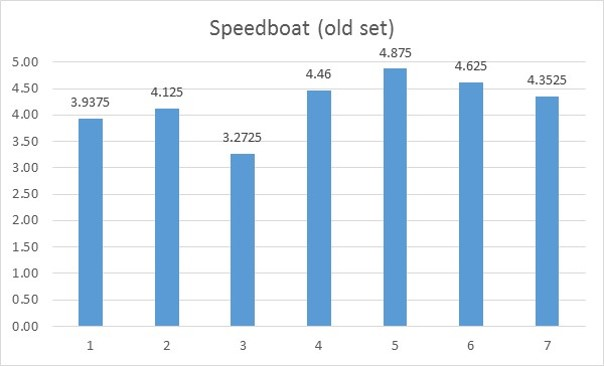
\includegraphics[width=1\textwidth]{charts/speedboatOldSet}
\end{figure}

As we can see on \autoref{fig:speedboatResultsOld}, the results are quite similar to each other. Also, the question "How would you evaluate the preparation of the game?" was excluded from the chart, because in the case of this study, it did not give any interesting characteristics. In this case, we are unable to actually retrieve any information, but what we do know is that the participants of the experiment agreed that the game had better results than the standard procedure. What is more, they thought that the discussions were successful. Not only were the employees willing to play the game but the work associated with the game had a positive impact on the team members and most importantly they said they would strongly recommend to permanently implement the game instead of using the standard procedure. On the other hand, some claimed it was hard to say
whether they gained any unique features thanks to the Speed boat game.

\subsection{Starfish Game deployment}

The "Starfish" game was also implemented in Team A (while they were evaluating theirs 32nd sprint) and Team B (whilst evaluating their 2nd sprint) using the old set of questions. The results for both teams are presented on \autoref{tab:groups-starTeamResults}. The first team playing this game were able to retrieve 8 things that should be started in order to make the sprint successful and the work easy, 1 thing that they should immediately stop doing, 4 things that they want to continue doing, because they are verified and good for the team and the project. They also found 4 things that should be made less and 3 things that should be done more. Team B retrieved 5 "start doing", 2 "stop doing", 2 "continue", 4 "less of" and 6 "more of". The game changed the perspective, so the participants were more creative and interested in a the game.

\begin{table}[!htbp]
	\caption{A bar graph depicting the results when deploying the Starfish game using the old set of questions}
	\label{tab:groups-starTeamResults}
	\begin{tabularx}{\textwidth}{|X|X|X|X|X|X|X|X|}
	\hline
		Group & Start doing & Stop doing & Continue & Less of &  Stop doing & Time & Comment\\ \hline
		Team A & 8 & 1 & 4 & 4 & 3 & 1 hour 45 minutes & 32nd sprint \\ \hline
		Team B & 5 & 2 & 2 & 4 & 6 & 1 hour 10 minutes & 2nd sprint \\ \hline
        Team C & N/A & N/A & N/A & N/A & N/A & N/A & N/A\\ \hline
	\end{tabularx}
\end{table}

\begin{figure}[!htbp]
\caption{Results of deploying starfish game using old set of questions}
\label{fig:starfishResultsOld}
\centering
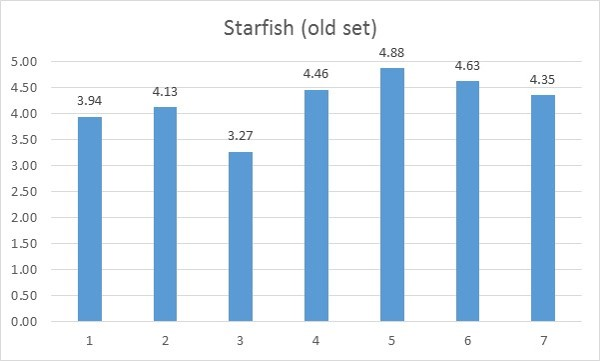
\includegraphics[width=1\textwidth]{charts/starfishOldSet}
\end{figure}

\autoref{fig:starfishResultsOld} presents the results of the "Starfish" deployment. As we can see, similarly to the "Speedboat" game results using the old question set, it is hard to retrieve useful data from this chart. The uniqueness of the features is hard to establish as in "Speedboat" deployment and the other results are more or less the same. 

\subsection{Discussion}
The chart on \autoref{fig:comparedResultsOld} presents a comparison of deploying the "Speedboat" and "Starfish" game. We can see that the results do not differ that much - this was the catalyst of actually changing the set of questions to retrieve more valuable characteristics. As the result we decided to ask more specific questions to retrieve better features. 


\begin{figure}[!htbp]
\caption{A comparison of deploying starfish and speedboat games using the old set of questions}
\label{fig:comparedResultsOld}
\centering
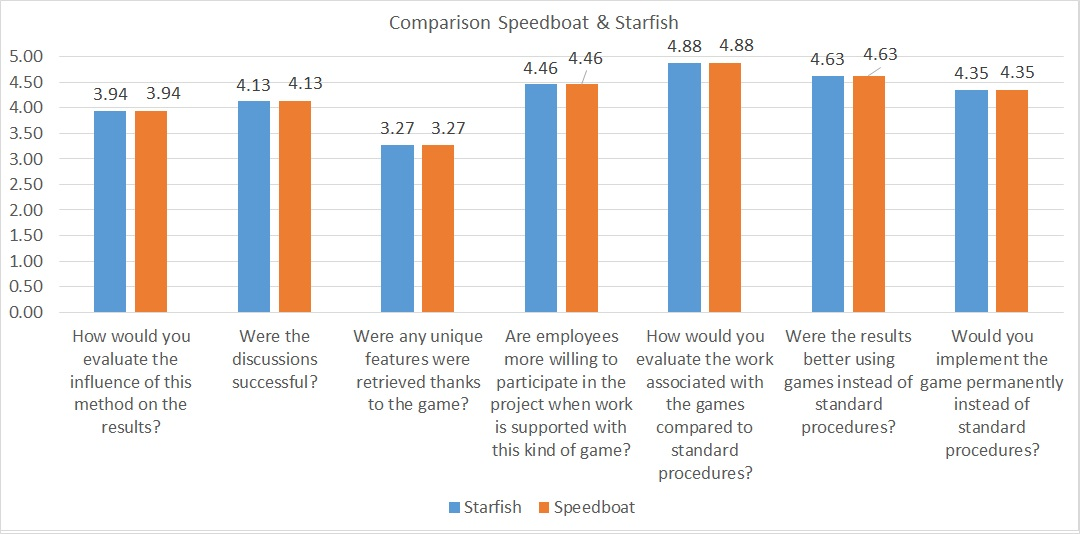
\includegraphics[width=1\textwidth]{charts/comparisonOldSet}
\end{figure}

\section{Second iteration}
\label{sec:secondIt}
\subsection{Speedboat Game deployment}

This test was deployed multiple times on every team that has been listed in \autoref{tab:groups-desc}. Using this game we are able to see that through a change of perspective, by not using standard procedures, we are able to look at things differently, realise what is pushing our boat forward, what might crush us and what is pulling us down. Thanks to the game, we have observed that the teams were more involved, motivated and eager to participate in retrospective game. \autoref{tab-groups-speedTeamResultsN} presents the results that were retrieved using the Speedboat technique by the performing the retrospective. In group B, the retrospective was performed for 45 minutes and in team C for 50 minutes. While team A was in their 33rd sprint, they were able to find 8 good things, 5 bad things and 3 to improve. Two sprints later, the results were as follows: 16 good things, 3 bad things and 4 things to improve. The team played the game for 1 hour 15 minutes on average. Team B played the game just once, while having a 3rd sprint, and it took them 45 minutes to successfully get 8 good things, 5 bad things and 6 things that needed improvement. The last team, team C, whilst having their 19th sprint, played the game once for 55 minutes and they retrieved 17 good things, 8 bad things and 5 things to improve.

\begin{table}[!htbp]
	\caption{Results of the Speedboat Game}
	\label{tab:groups-speedTeamResultsN}
	\begin{tabularx}{\textwidth}{|X|X|X|X|X|X|}
	\hline
		Group &  The cloud & The rocks & The anchor & Time & Comment\\ \hline
		Team A & 8 & 5 & 3 & 1 hour 20 minutes & 33rd sprint \\ \hline
		Team A & 16 & 3 & 4 & 1 hour 10 minutes & 35th sprint\\ \hline
		Team B & 8 & 5 & 6 & 45 minutes & 3rd sprint\\ \hline
        Team C & 17 & 8 & 5 & 50 minutes & 19th sprint\\ \hline
	\end{tabularx}
\end{table}

\autoref{fig:speedboatLive} presents the "Speedboat" game deployment. Every single game described in this chapter was documented with a picture and the feedback from the team.

\begin{figure}[!htbp]
\caption{Speedboat deployment}
\label{fig:speedboatLive}
\centering
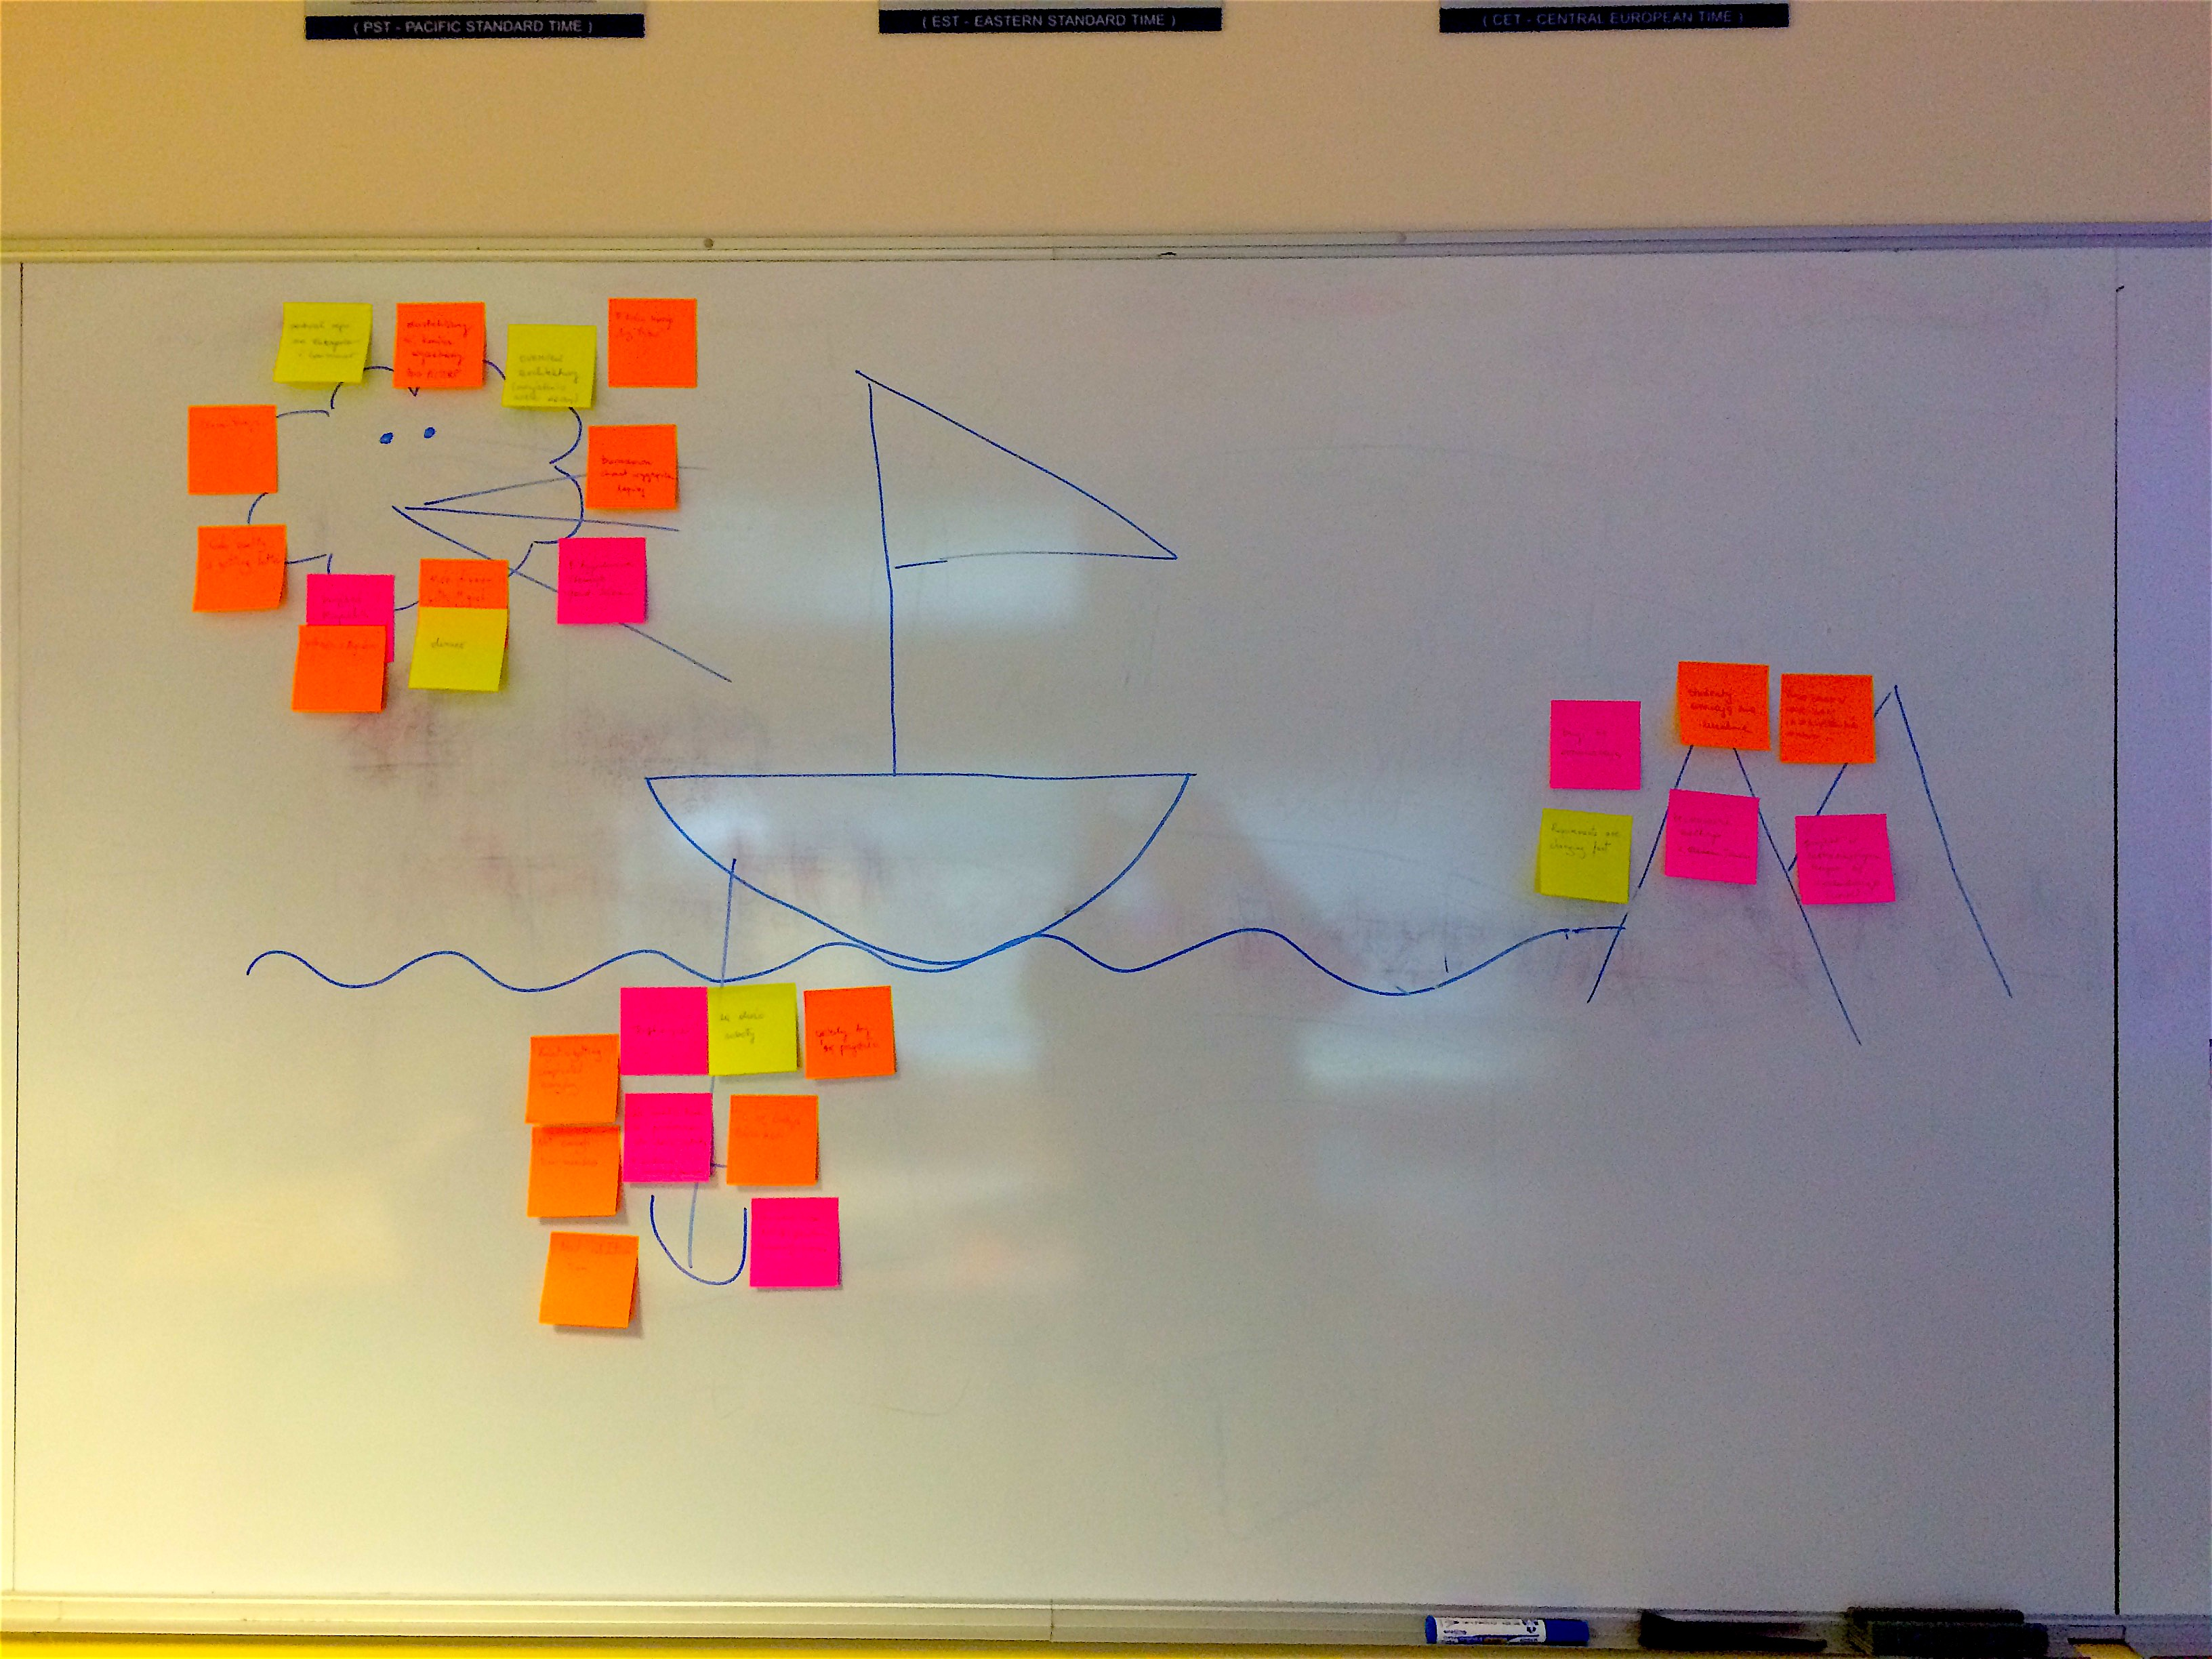
\includegraphics[width=1\textwidth]{live/speedboatLive}
\end{figure}

\begin{figure}[!htbp]
\caption{A bar graph depicting the results when deploying the Speedboat game using the new set of questions}
\label{fig:speedboatResultsNew}
\centering
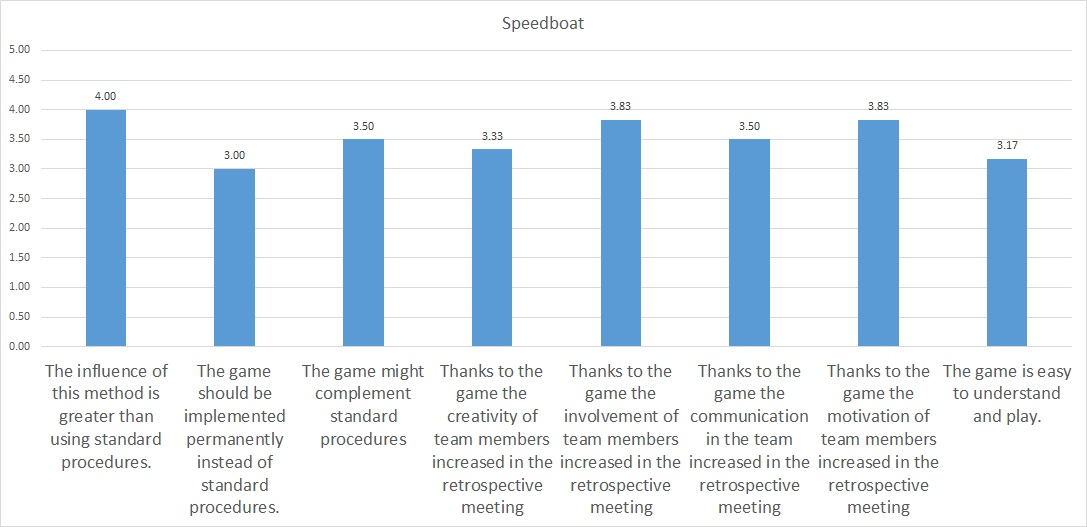
\includegraphics[width=1\textwidth]{charts/speedboatNewSet}
\end{figure}

Analysing the results from \autoref{fig:speedboatResultsNew}, we were able to retrieve that through playing the game, the team was seeing a better influence on the retrospective meeting, but surprisingly, it was hard for them to decide whether they would like to play this game permanently during the next meetings. The probable cause of the latter is that even though the game is fun and useful, it should not be used on every retrospective. This is due the monotony nature, which we would like to reduce. They could not also decide definitely, but were more convinced than in the previous question, that this game might complement standard procedures. Regarding the characteristics of the game, they were almost definitely convinced that they agree on statements about motivation and involvement of participants while playing "Speedboat". However, they were less convinced about communication being increased and they were also not convinced about the team members' creativity. Moreover, what is actually surprising is that they could not decide on the level of difficulty in terms of understanding the game. 
\subsection{Starfish Game deployment}

The "Starfish" game was a big surprise for all the teams due to a drastic change in perspective. The five fields which had to be filled created multiple discussions. The game was implemented in teams A, B and C. None of the participants in these teams were familiar with this game, so because of the complexity in the preparation of the game, explaining the rules and giving the participants the time to familiarize with the new approach, this made the meeting last much longer. The data presented on \autoref{tab:groups-starTeamResultsN} shows the results retrieved by the teams in the retrospective meeting using the described game used in this subsection. On average, team A finished the meeting after 1 hour 45minutes. They played the game after their 36th sprint and the game resulted in 9 things that they should start doing, 3 stop doing, 3 continue, 5 less and 2 more. Team B was in their 4th sprint and finished the game in 45minutes. They attained 6 things that may increase their effectiveness and are good for the team, and as a result they should start doing them, 1 that is stopping them and they should dispose of it, 7 things that are being already done in the team and they want to continue performing them, 6 things that the team should do less and 1 thing that should be done more often. While having the 21st sprint, team C retrieved 6 start doing things, 4 stop doing, 2 continue, 3 less of and 2 more of. The game lingered for 1hour 10 minutes. It was an interesting experience to work with teams which are so involved in the retrospective meeting.

\begin{table}[!htbp]
	\caption{Results of the Starfish Game}
	\label{tab:groups-starTeamResultsN}
	\begin{tabularx}{\textwidth}{|X|X|X|X|X|X|X|X|}
	\hline
		Group & Start doing & Stop doing & Continue & Less of &  More of & Time & Comment\\ \hline
		Team A & 9 & 3 & 3 & 5 & 2 & 1 hour 45 minutes & 36th sprint \\ \hline
		Team B & 6 & 1 & 7 & 6 & 1 & 45 minutes & 4th sprint\\ \hline
        Team C & 6 & 4 & 2 & 3 & 2 & 1 hour 10 minutes & 21st sprint\\ \hline
	\end{tabularx}
\end{table}

\autoref{fig:starfishLive} presents live deployment of the "Starfish" game.

\begin{figure}[!htbp]
\caption{Starfish deployment}
\label{fig:starfishLive}
\centering
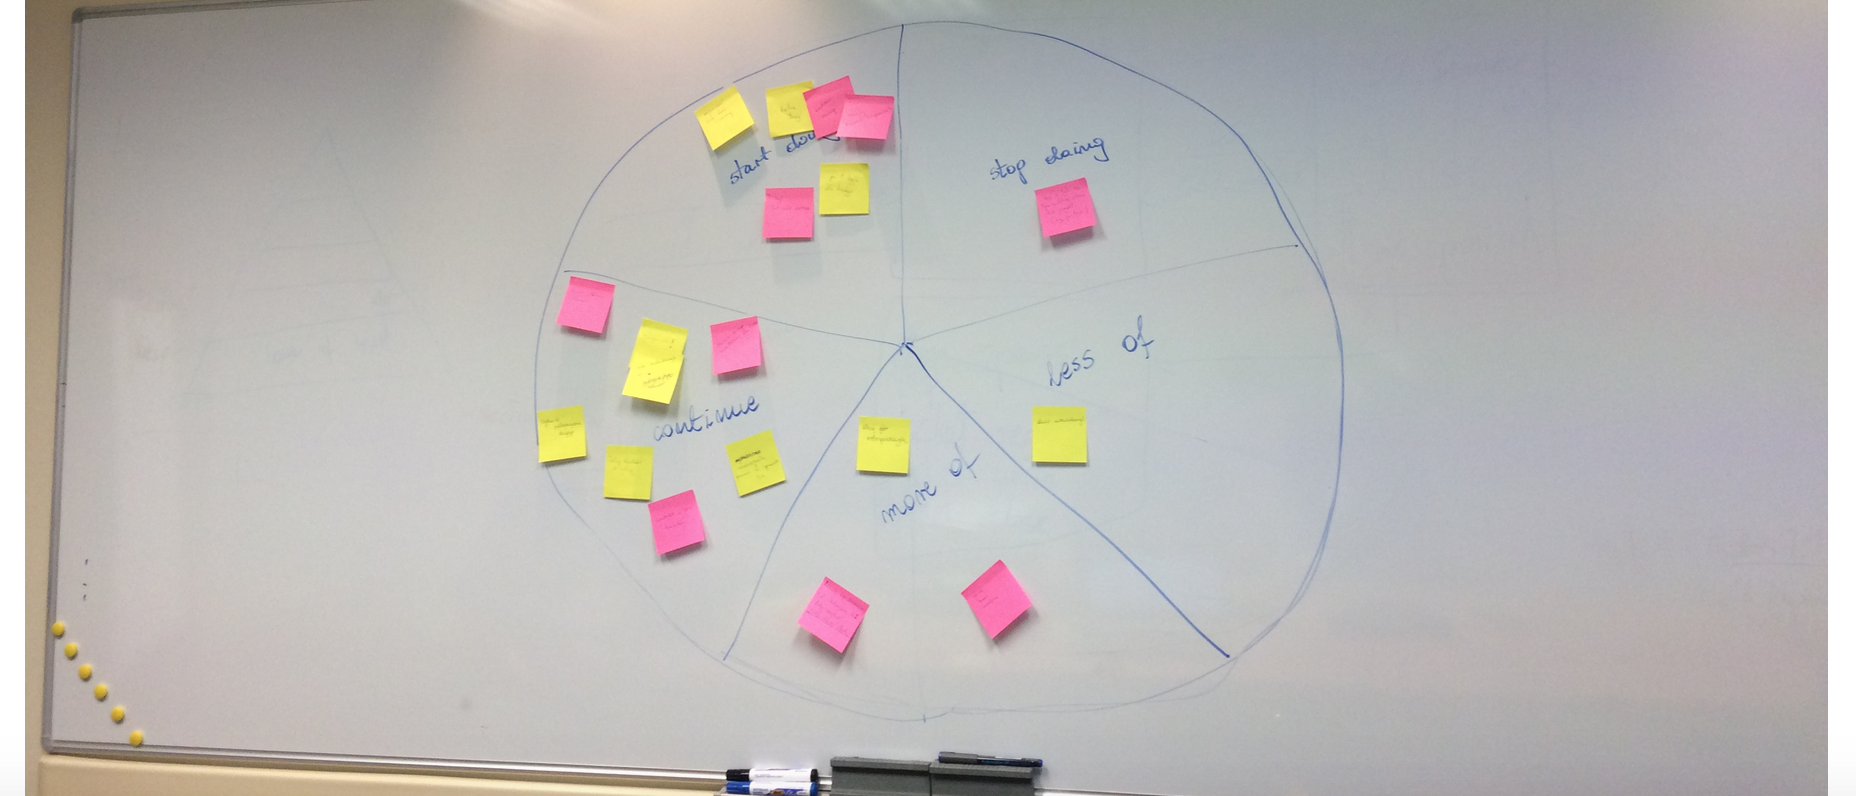
\includegraphics[width=1\textwidth]{live/starfishLive}
\end{figure}


The results in \autoref{fig:starfishResultsNew} represent the feedback retrieved from the team members listed in \autoref{tab:groups-desc} upon playing the "Starfish" game. The participants decided that they agree that the game should be permamently implemented in retrospective meetings. Moreover, based on their opinion, the results using this approach is greater than using standard procedures. Regarding the ease of the game, after preparation and discussing the rules, they decided that even though the game is complex, they understood it clearly after being presented with a proper introduction. A majority of the participants answered that involvement is a characteristic that could be retrieved from the "Starfish" game. Regarding the motivation and creativity on the other hand, the features that can also be increased using this approach, probably because of the innovation of this game. The groups would rather use this game permanently than as a supplement of standard procedures. Most of the team members were not convinced though whether communication was actually improved through playing this game.

\begin{figure}[!htbp]
\caption{A bar graph depicting the results when deploying the Starfish game using the new set of questions}
\label{fig:starfishResultsNew}
\centering
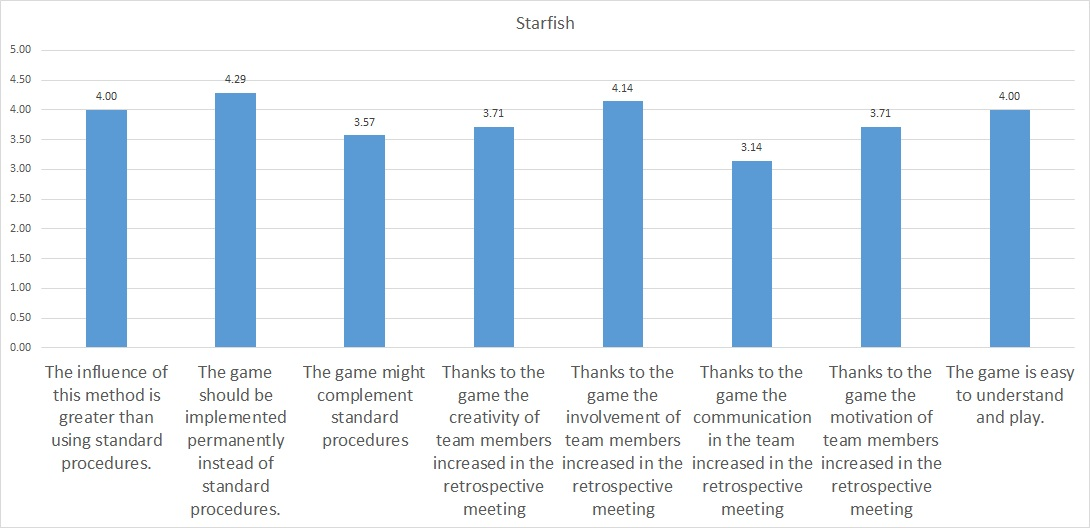
\includegraphics[width=1\textwidth]{charts/starfishNewSet}
\end{figure}

\subsection{Glad/Mad/Sad Game deployment}

Glad/Mad/Sad, also known as Happy/Sad/Angry game, was deployed in groups B and C, but because internal changes cooperation with team A was not possible anymore. The Glad/Mad/Sad was not a surprise for the teams. The approach of this game is very similar to the standard one, but if you have a choice, it is better to use the Glad/Mad/Sad technique rather than the standard Good Things, Bad Things, Things to Improve technique in order to diversify the retrospective meeting. Both teams played once for approximately 45 minutes with team B having their 5th sprint, and team C their 20th sprint. \autoref{tab:groups-gmsResultsN} shows the results which were retrieved by the teams. Team A was able to get 8 things that made them glad, 7 mad and 2 sad and team C was able to get 10, 9 and 14 respectively.

\begin{table}[!htbp]
	\caption{Results of the Glad, Mad, Sad Game}
	\label{tab:groups-gmsResultsN}
	\begin{tabularx}{\textwidth}{|X|X|X|X|X|X|}
	\hline
		Group & Glad & Mad & Sad & Time & Comment\\ \hline
		Team A & N/A & N/A & N/A & N/A & N/A\\ \hline
		Team B & 8 & 7 & 2 & 40 minutes & 5th sprint\\ \hline
        Team C & 10 & 9 & 14 & 50 minutes & 20th sprint\\ \hline
	\end{tabularx}
\end{table}

On the \autoref{fig:hsaLive} we can see the deployment of the "Glad, Mad, Sad" Game in Intel Technology Poland in Gdańsk.

\begin{figure}[!htbp]
\caption{Glad, Mad, Sad deployment}
\label{fig:hsaLive}
\centering
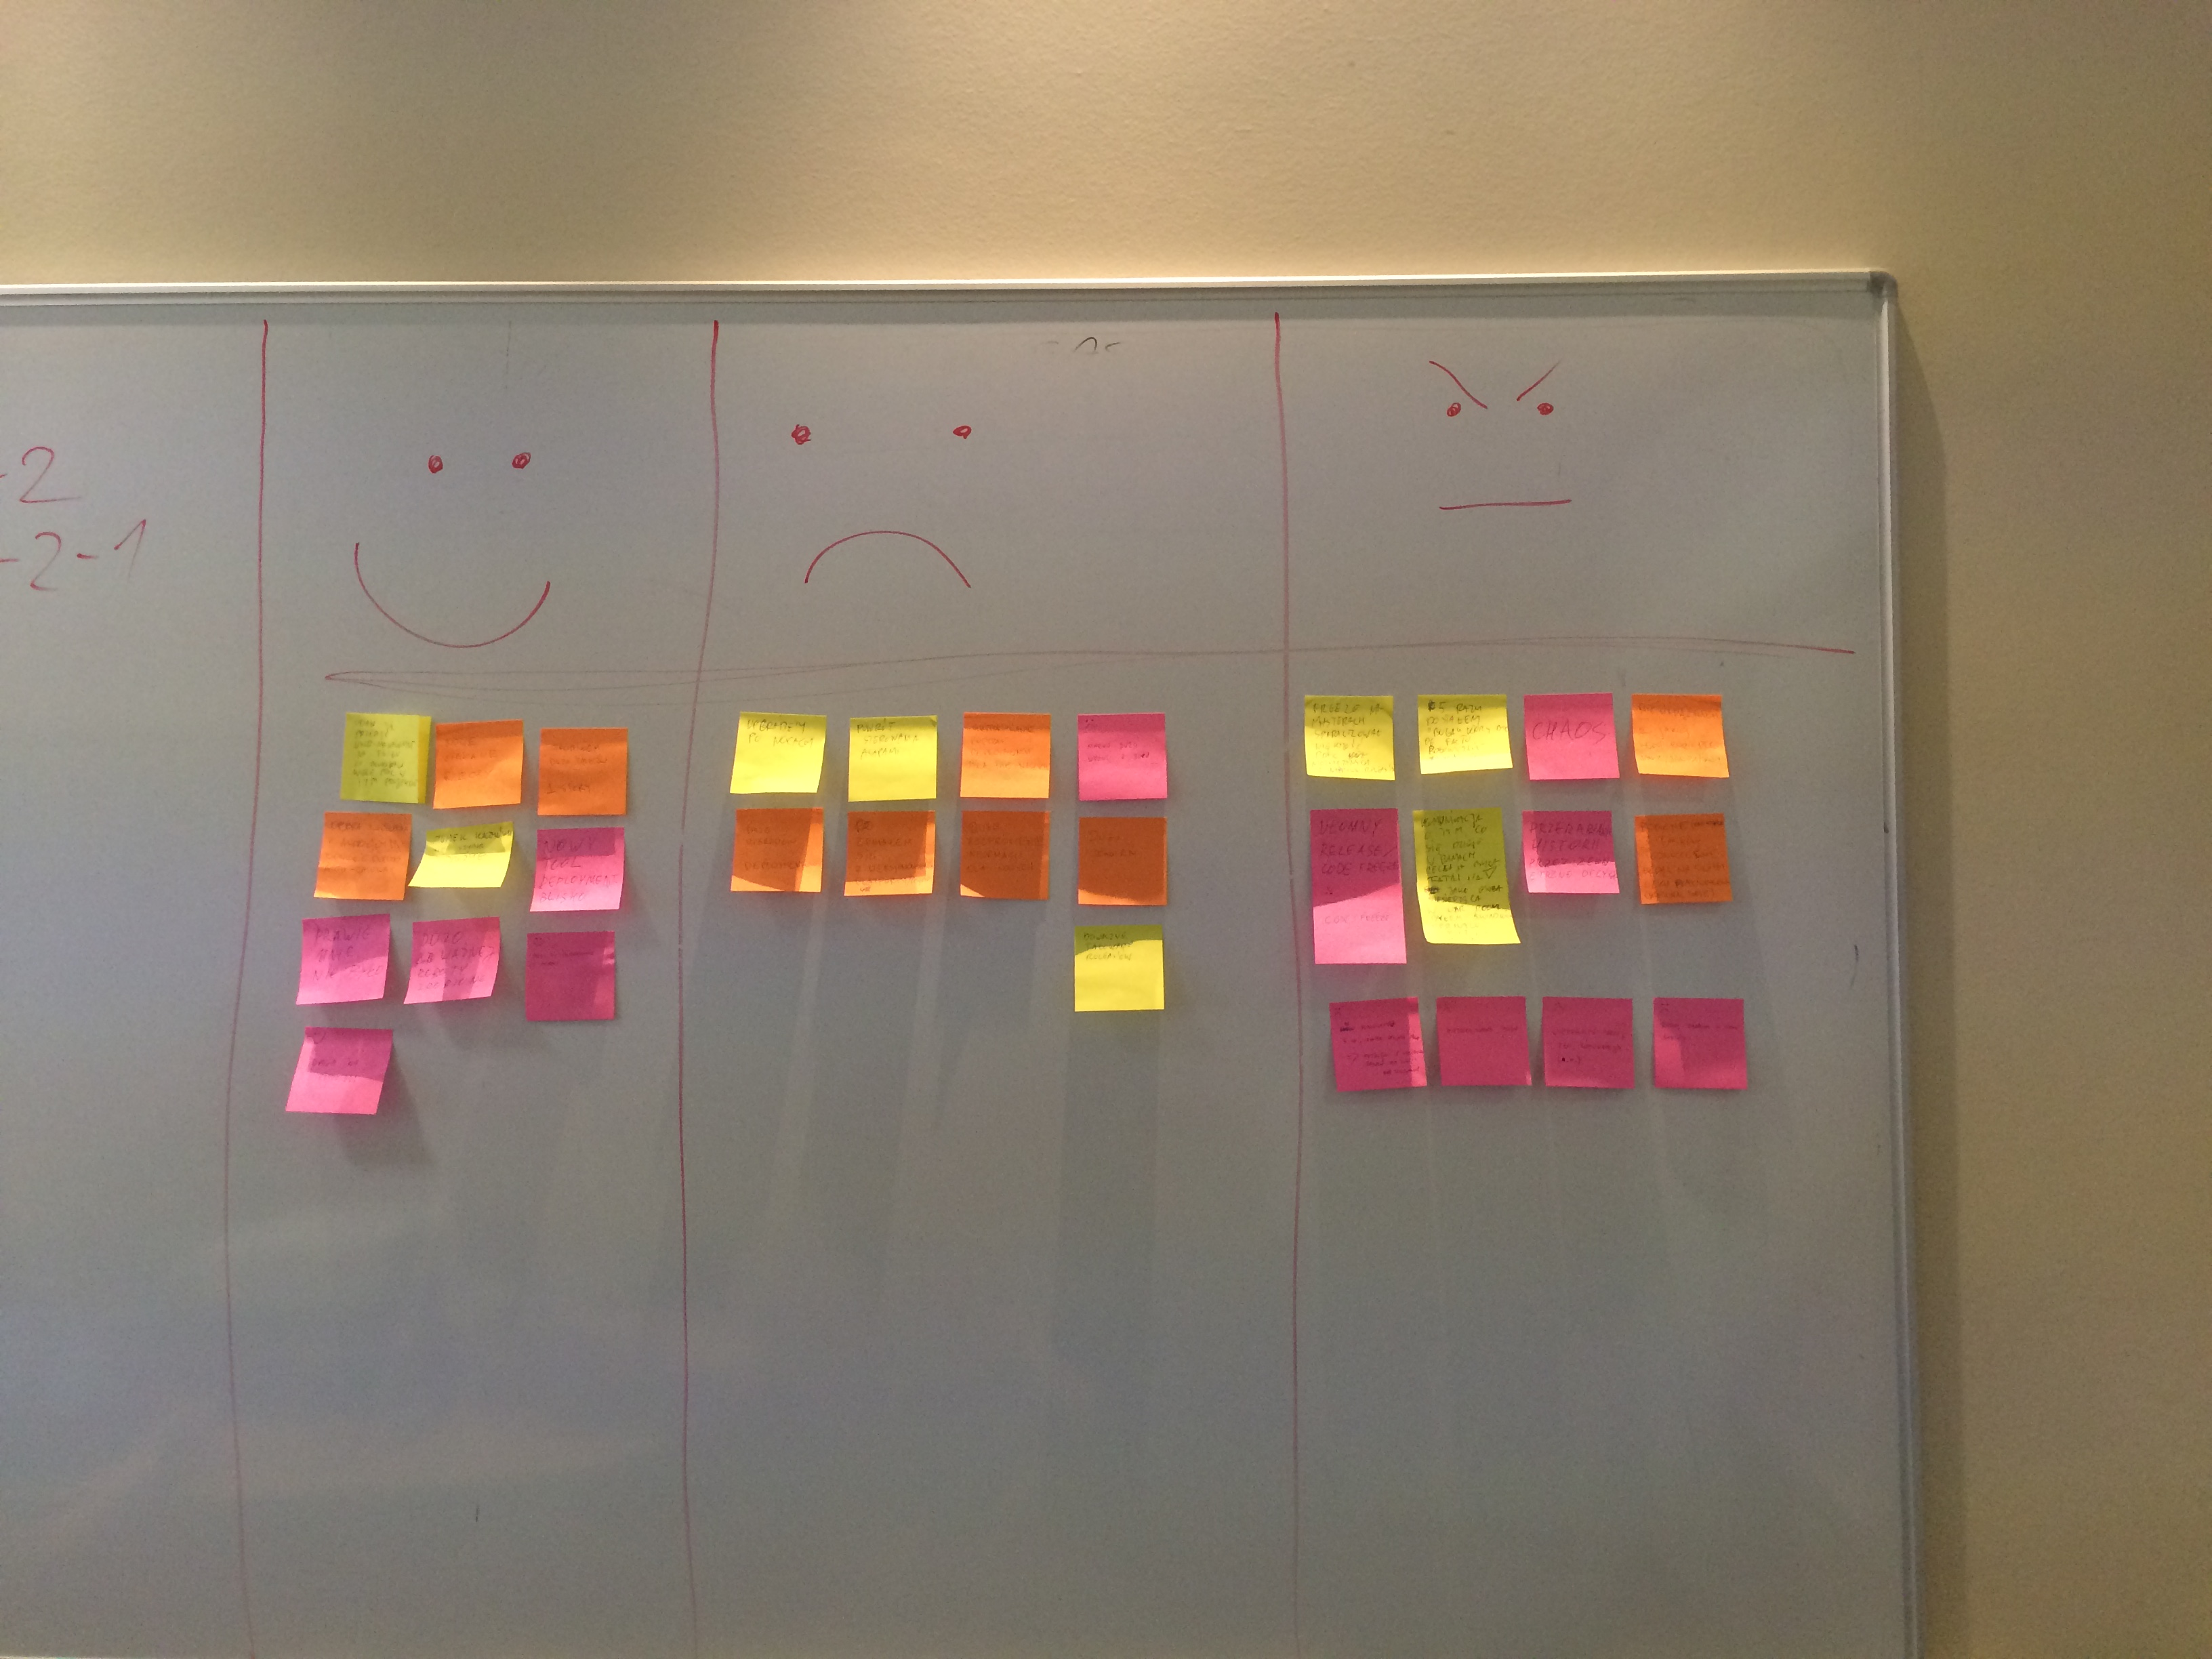
\includegraphics[width=1\textwidth]{live/hsaLive}
\end{figure}

\autoref{fig:gmsResultsNew} presents the results of the Glad/Mad/Sad game deployment. The highest result was retrieved in the third and eighth question and indicates that participants agree on the fact that this technique might complement standard procedures and is easy to understand. The members of the experiment are also rather convinced that the game had increased the teams' creativity, which proves a previously presented thesis that it is better to use the Glad/Mad/Sad approach, rather than the standard technique. In terms of the influence of game on improving the results, the participants were undecided on whether the game should be implemented permanently and whether the involvement of team members is increased in the retrospective meeting. The attendees of the experiments agreed that communication and motivation of team members was not influenced by this technique.    

\begin{figure}[!htbp]
\caption{A bar graph depicting the results when deploying the Glad/Mad/Sad game using the new set of questions}
\label{fig:gmsResultsNew}
\centering
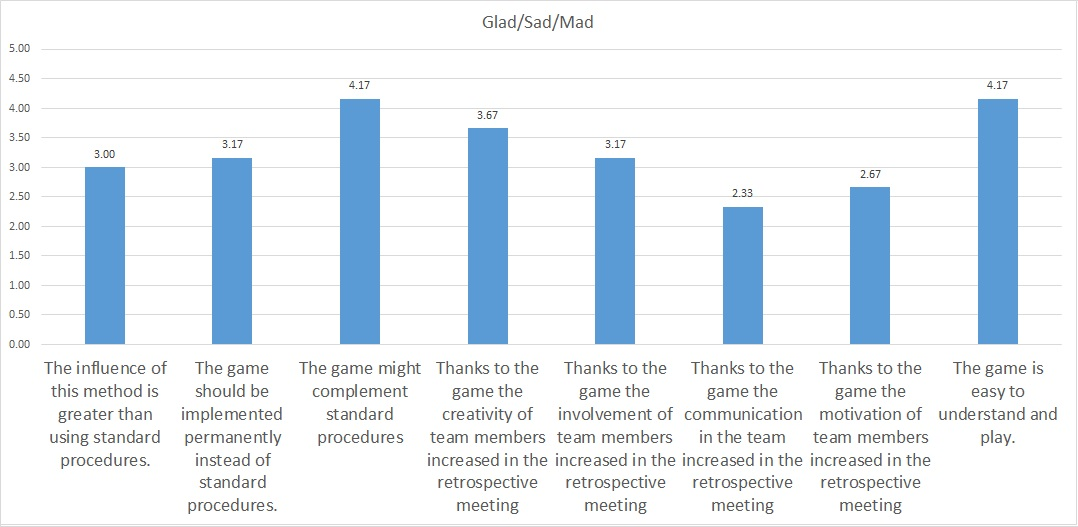
\includegraphics[width=1\textwidth]{charts/gmdNewSet}
\end{figure}

\subsection{Mood and improvements Game deployment}
\autoref{fig:moodLive} presents the deployment of the "Mood and improvements" game that have been created in collaboration with Intel Technology Teams. We merged the "Glad, Mad, Sad" game with two fields to indicate ideas for improvements and appreciations amongst team members. 

\begin{figure}[!htbp]
\caption{Mood and improvements game deployment}
\label{fig:moodLive}
\centering
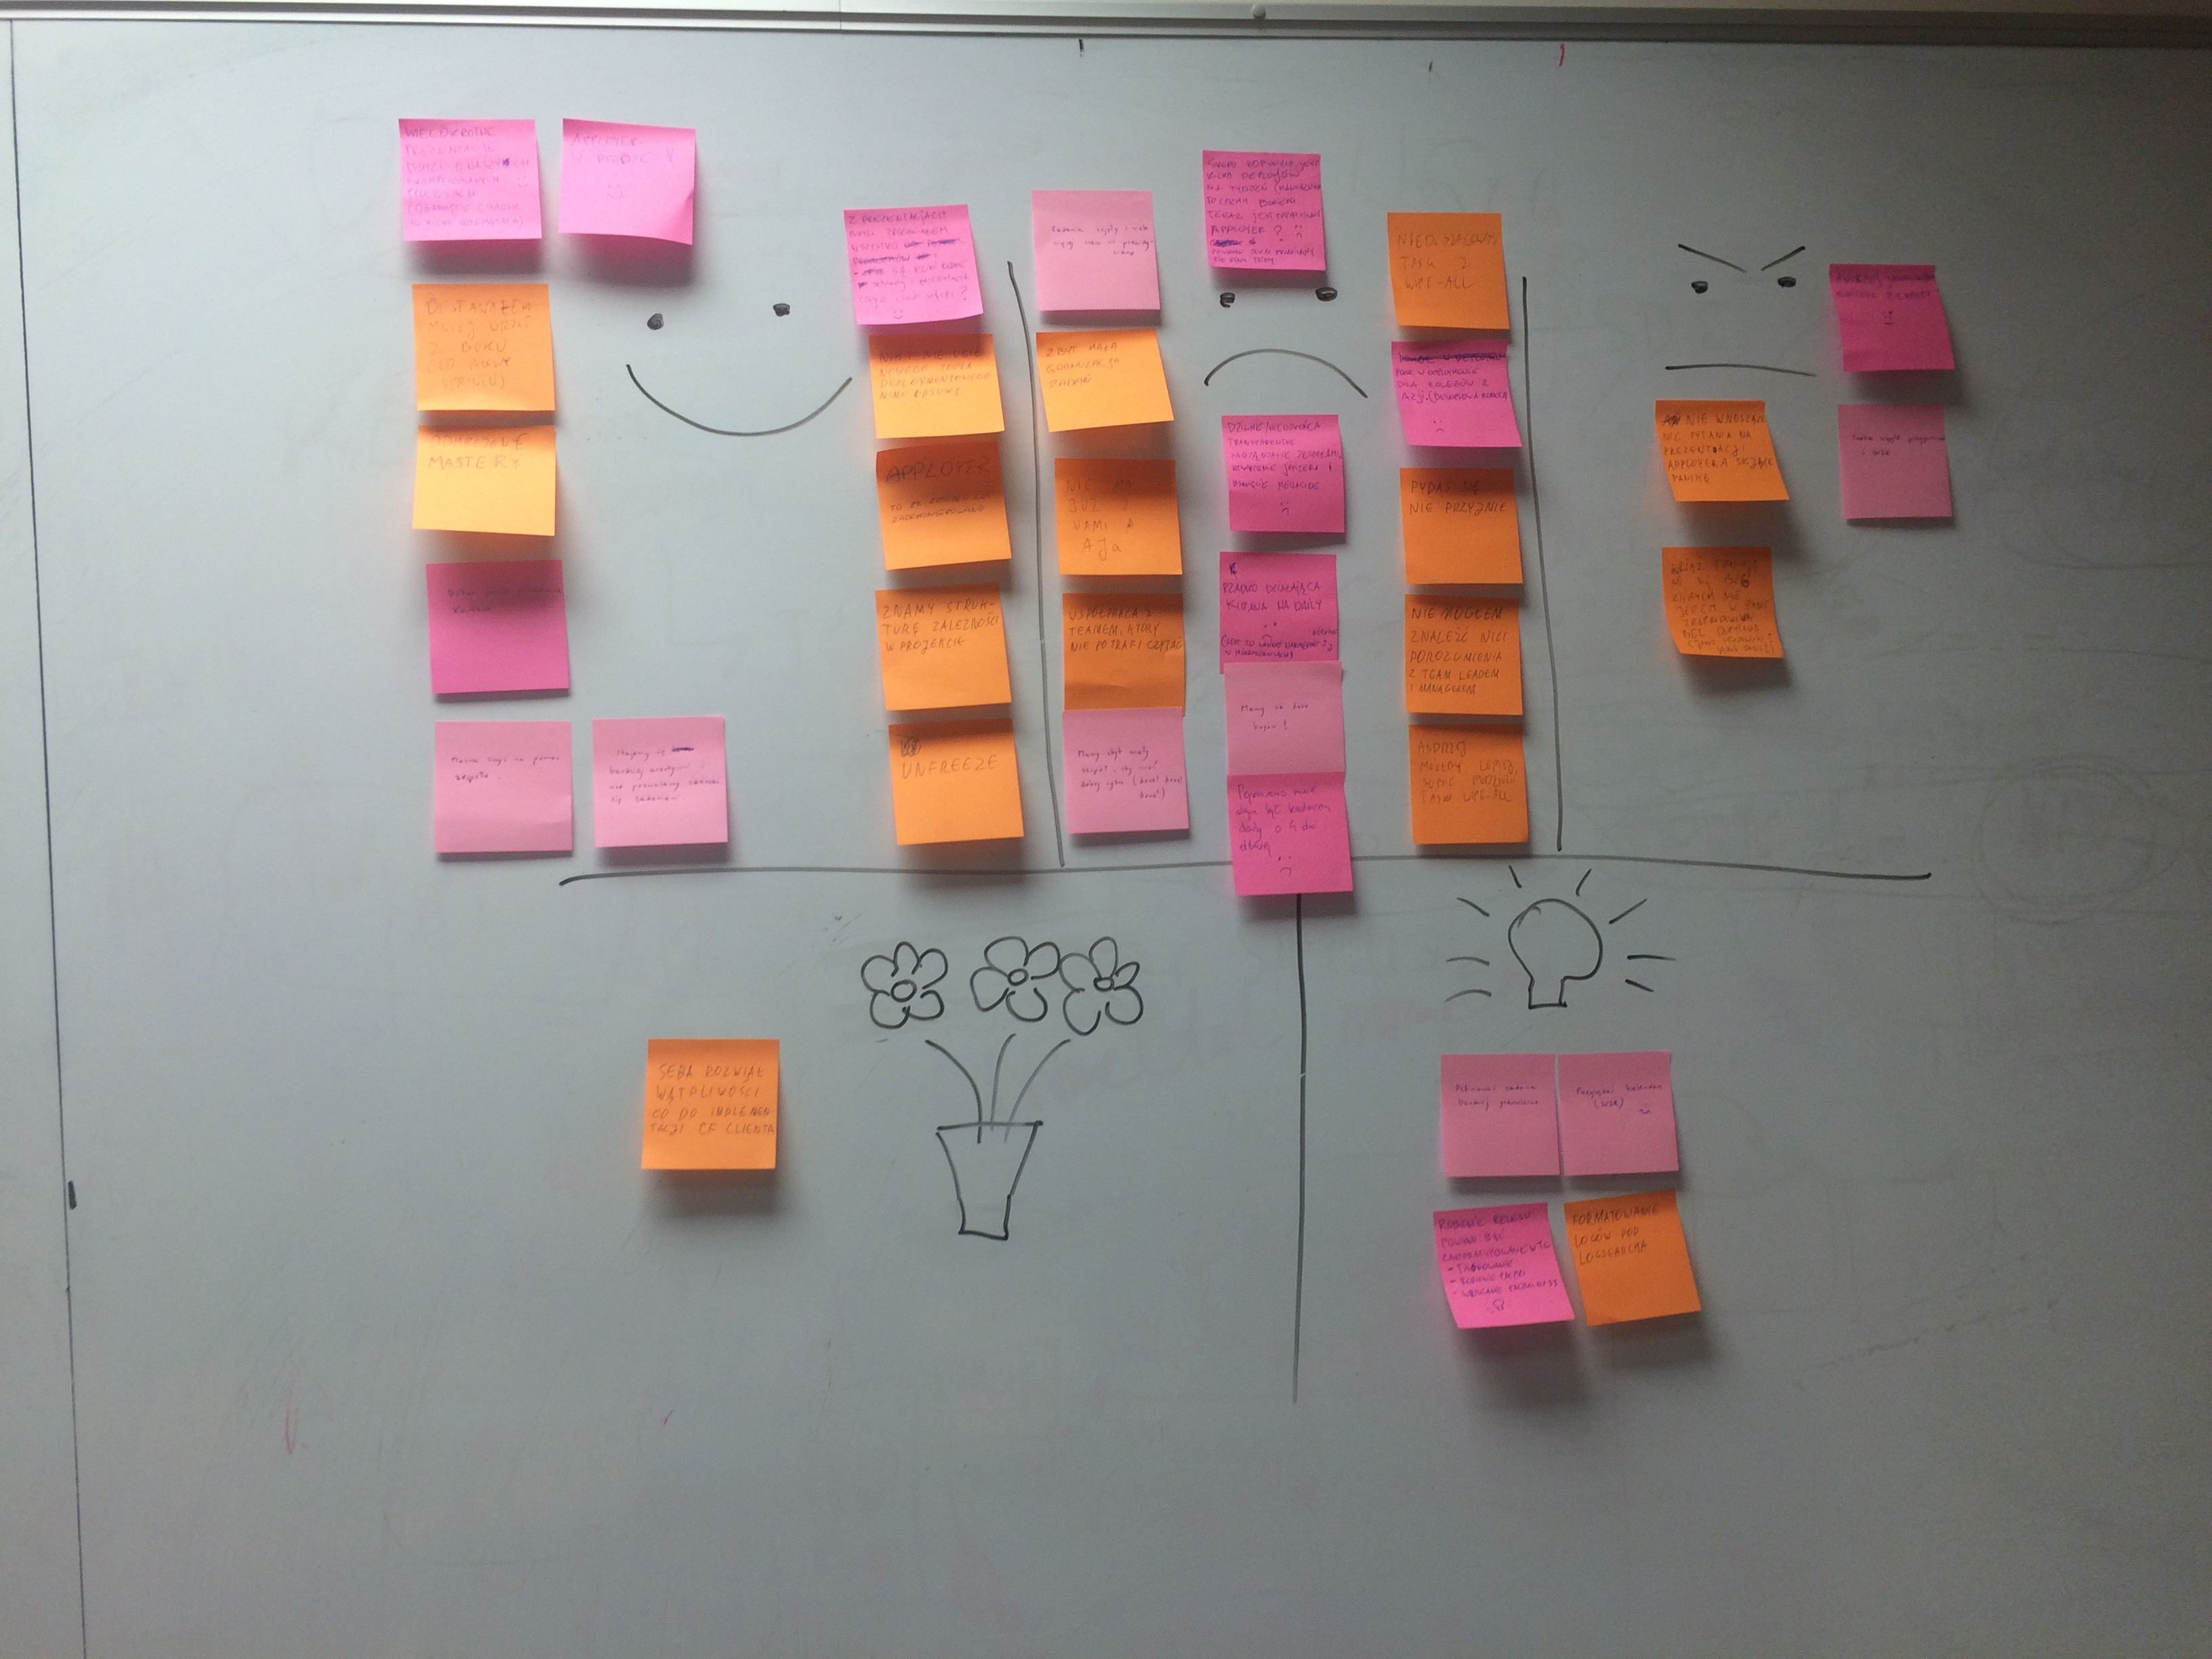
\includegraphics[width=1\textwidth]{live/moodLive}
\end{figure}

\autoref{tab:groups-moodTeamResultsN} presents the results of the Mood and Improvements Game implementation. On average, team B played the game twice for 45 minutes and in their 6th sprint retrieved 6 things that made them glad, 3 mad and 6 sad. They also had 3 ideas for improvement and 4 appreciations. In the 9th sprint, they found 13 things that made them glad, 2 mad and 2 sad, 3 ideas for improvement and 1 appreciation. The second team that participated in the research was team C and in their 22nd sprint, they were able to get 12 good things, 16 bad things, 4 things to improve, 4 ideas for enhancement and 1 appreciation. This took them 50 minutes to finish the game.

\begin{table}[!htbp]
	\caption{Results of the Mood and Improvements Game}
	\label{tab:groups-moodTeamResultsN}
	\begin{tabularx}{\textwidth}{|X|X|X|X|X|X|X|X|}
	\hline
		Group & Glad & Mad & Sad & Ideas for improvement & Appreciations & Time & Comments\\ \hline
		Team A & N/A & N/A & N/A & N/A & N/A & N/A & N/A \\ \hline
		Team B & 6 & 3 & 6 & 4 & 4 & 35 minutes & 6th sprint \\ \hline
		Team B & 13 & 2 & 2 & 3 & 1 & 55 minutes & 9th sprint \\ \hline
		Team C & 12 & 16 & 4 & 4 & 1 & 50 minutes & 22nd sprint\\ \hline
	\end{tabularx}
\end{table}

\autoref{fig:moodResultsNew} presents the results of feedback received from the participants. The chart indicates that the game was easy to understand and might complement standard procedures. The participants also agreed on the fact that the game increases creativity, communication and involvement. Moreover, they agreed that the game had a better influence on the results compared to standard procedures and are willing to permanently implement it into the retrospective meeting. The only characteristic that attendants of the experiment cannot decide on is, whether the technique increases motivation.

\begin{figure}[!htbp]
\caption{A bar graph depicting the results when deploying the Mood and Improvements game using the new set of questions}
\label{fig:moodResultsNew}
\centering
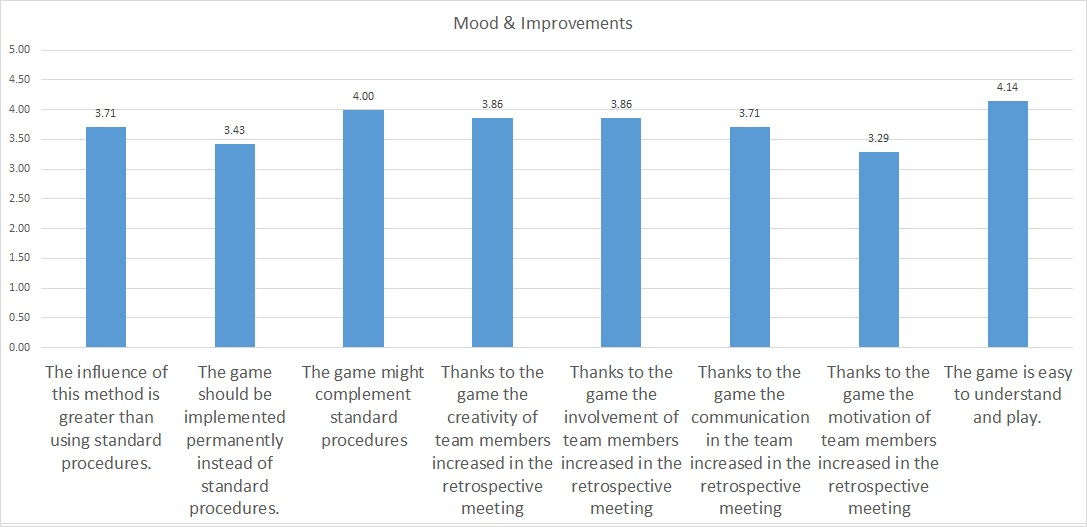
\includegraphics[width=1\textwidth]{charts/moodNewSet}
\end{figure}

\subsection{5L's Game deployment}
The "5L: Liked, Learned, Lacked, Longed for, Loathed" has been created in collaboration with Intel Technology Poland teams, using as a archetype game "4 L's". This approach changes the perspective, shows the participants a different point of view and enables them to learn more about other team members, for example what they learned in the past iteration or what was actually important for them what was done, but they have an idea to improve the current technique used in the project. There are two ways of playing the game that were deployed in the teams. The first one is shown on the \autoref{fig:5lLive}, the areas are arranged in the circle.

\begin{figure}[!htbp]
\caption{5 L's game deployment}
\label{fig:5lLive}
\centering
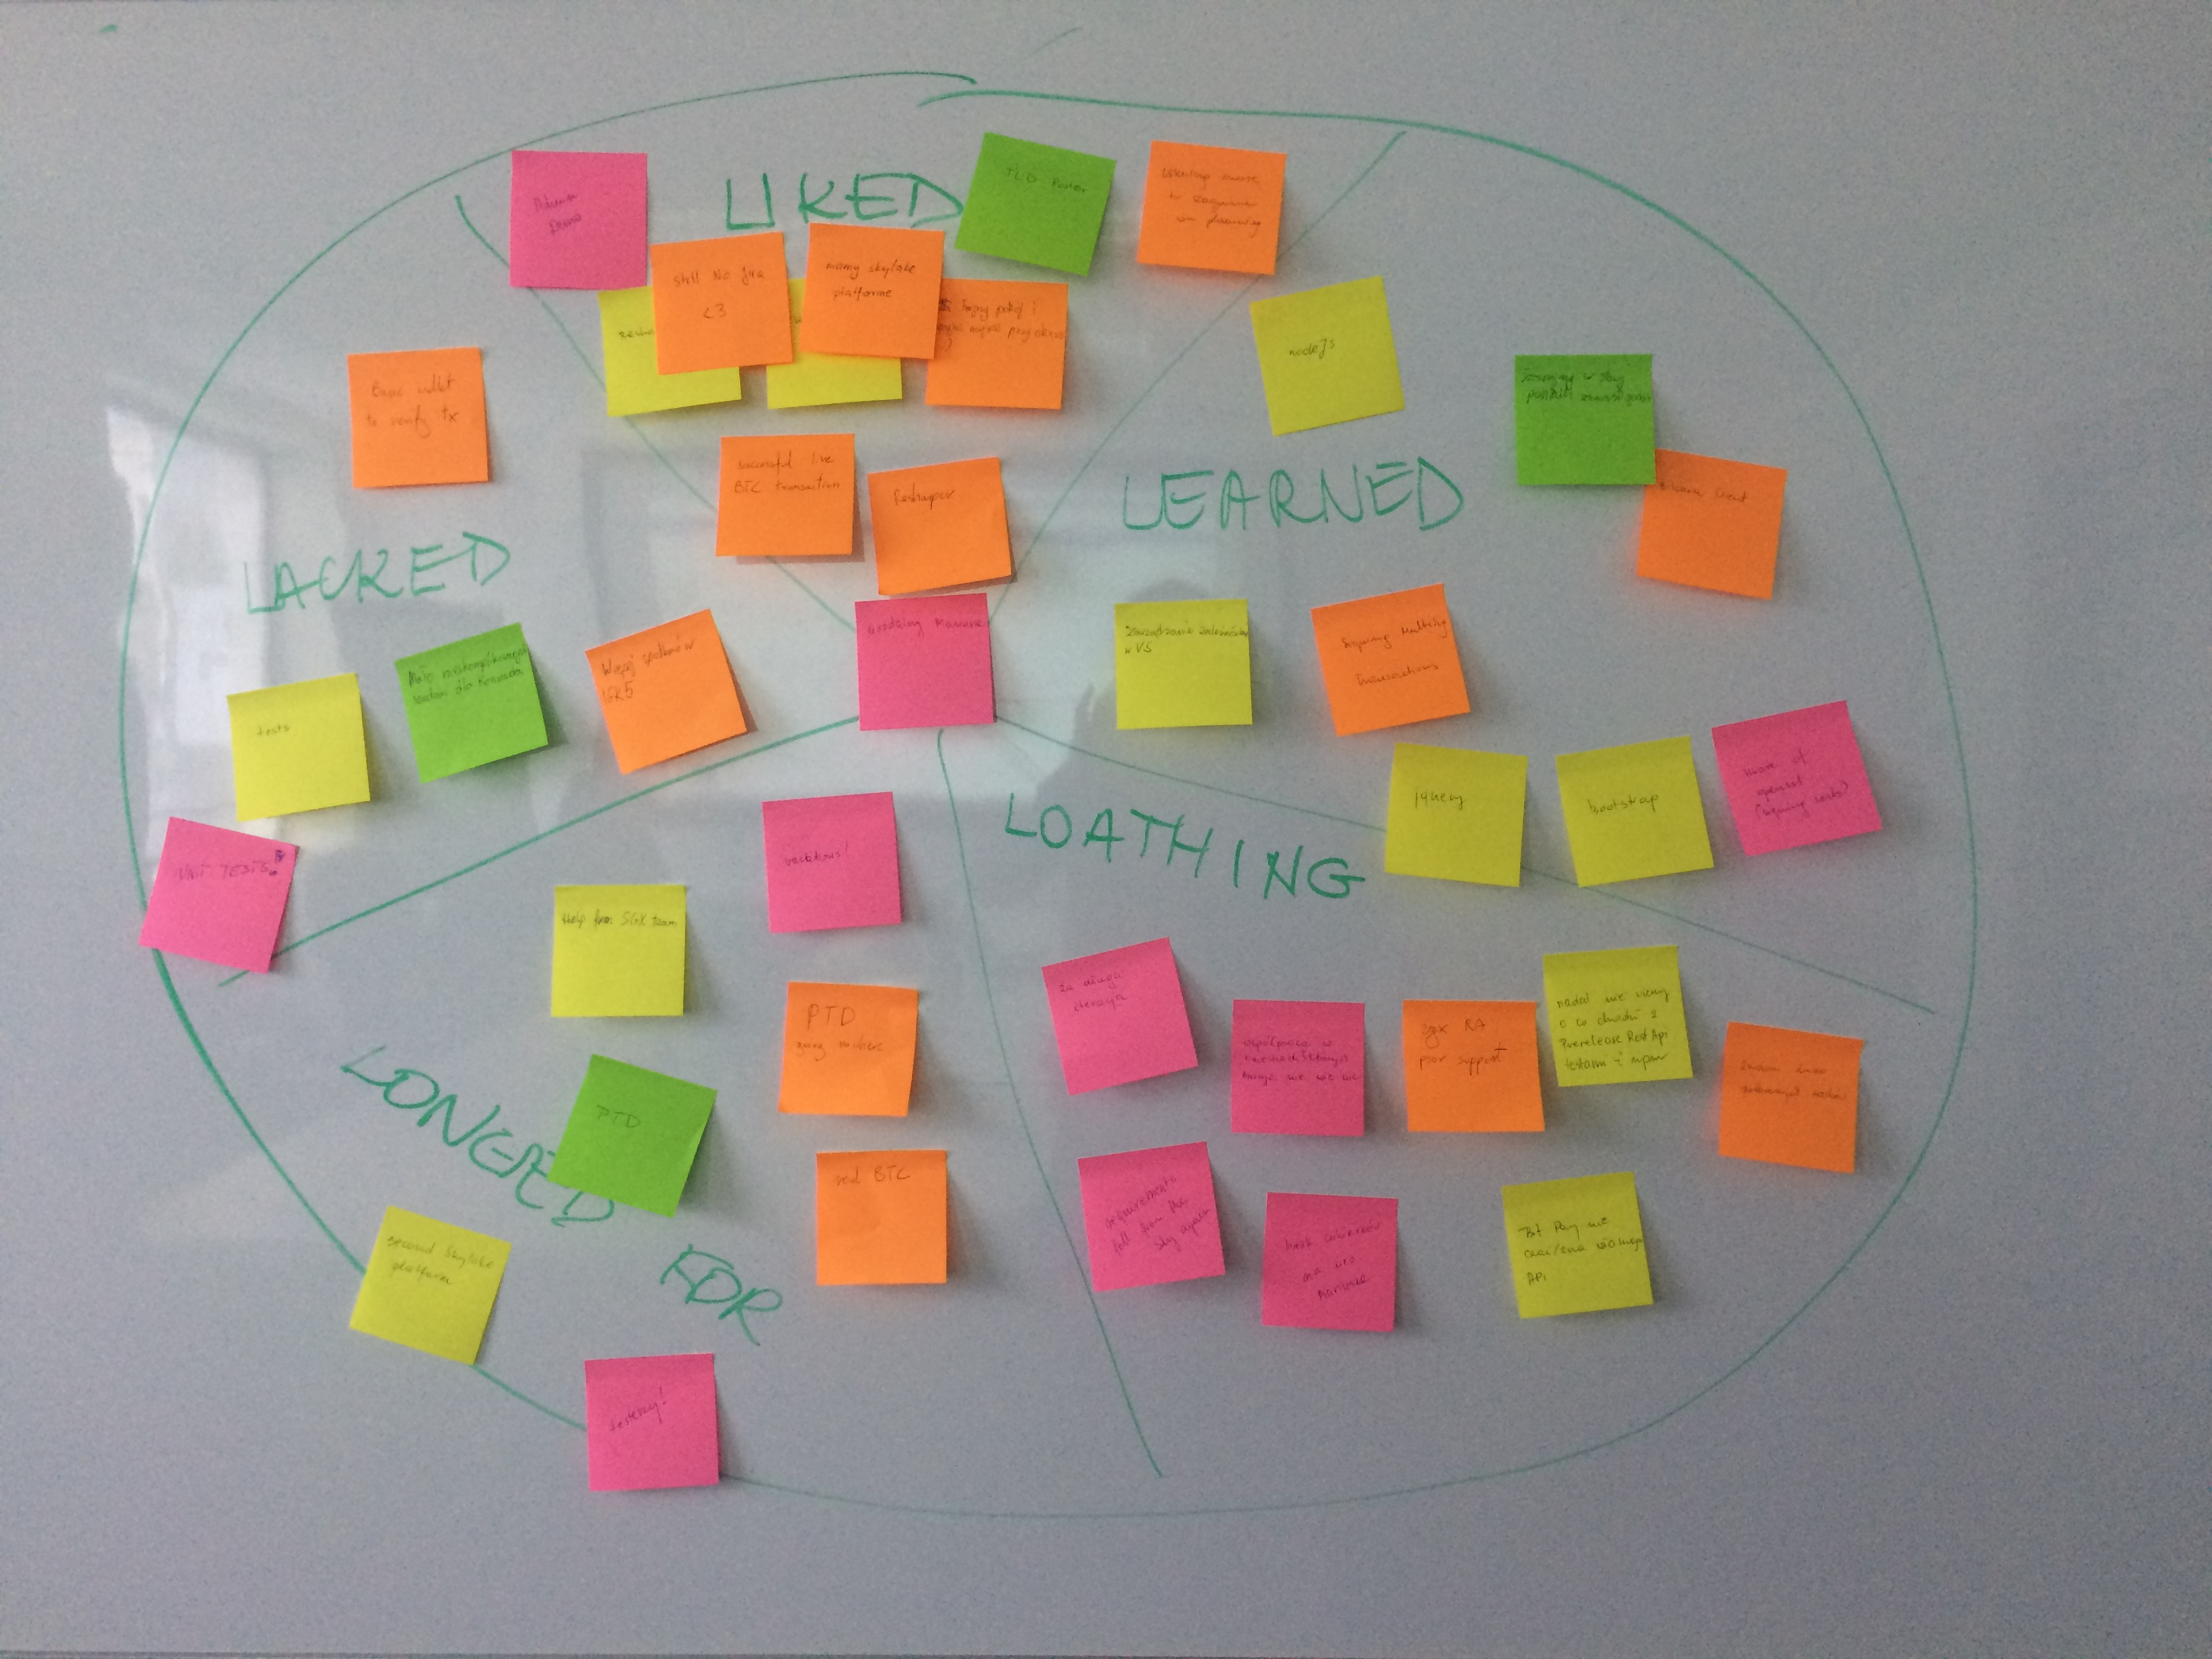
\includegraphics[width=1\textwidth]{live/5lLive}
\end{figure}
The second one is presented on \autoref{fig:5lLive2} and in this approach we arranged the fields in columns, what is more we assigned sticky-notes colors to particular area, this way we were able to see a clearer picture, where the most features are condensed. 
\begin{figure}[!htbp]
\caption{5 L's game deployment different representation}
\label{fig:5lLive2}
\centering
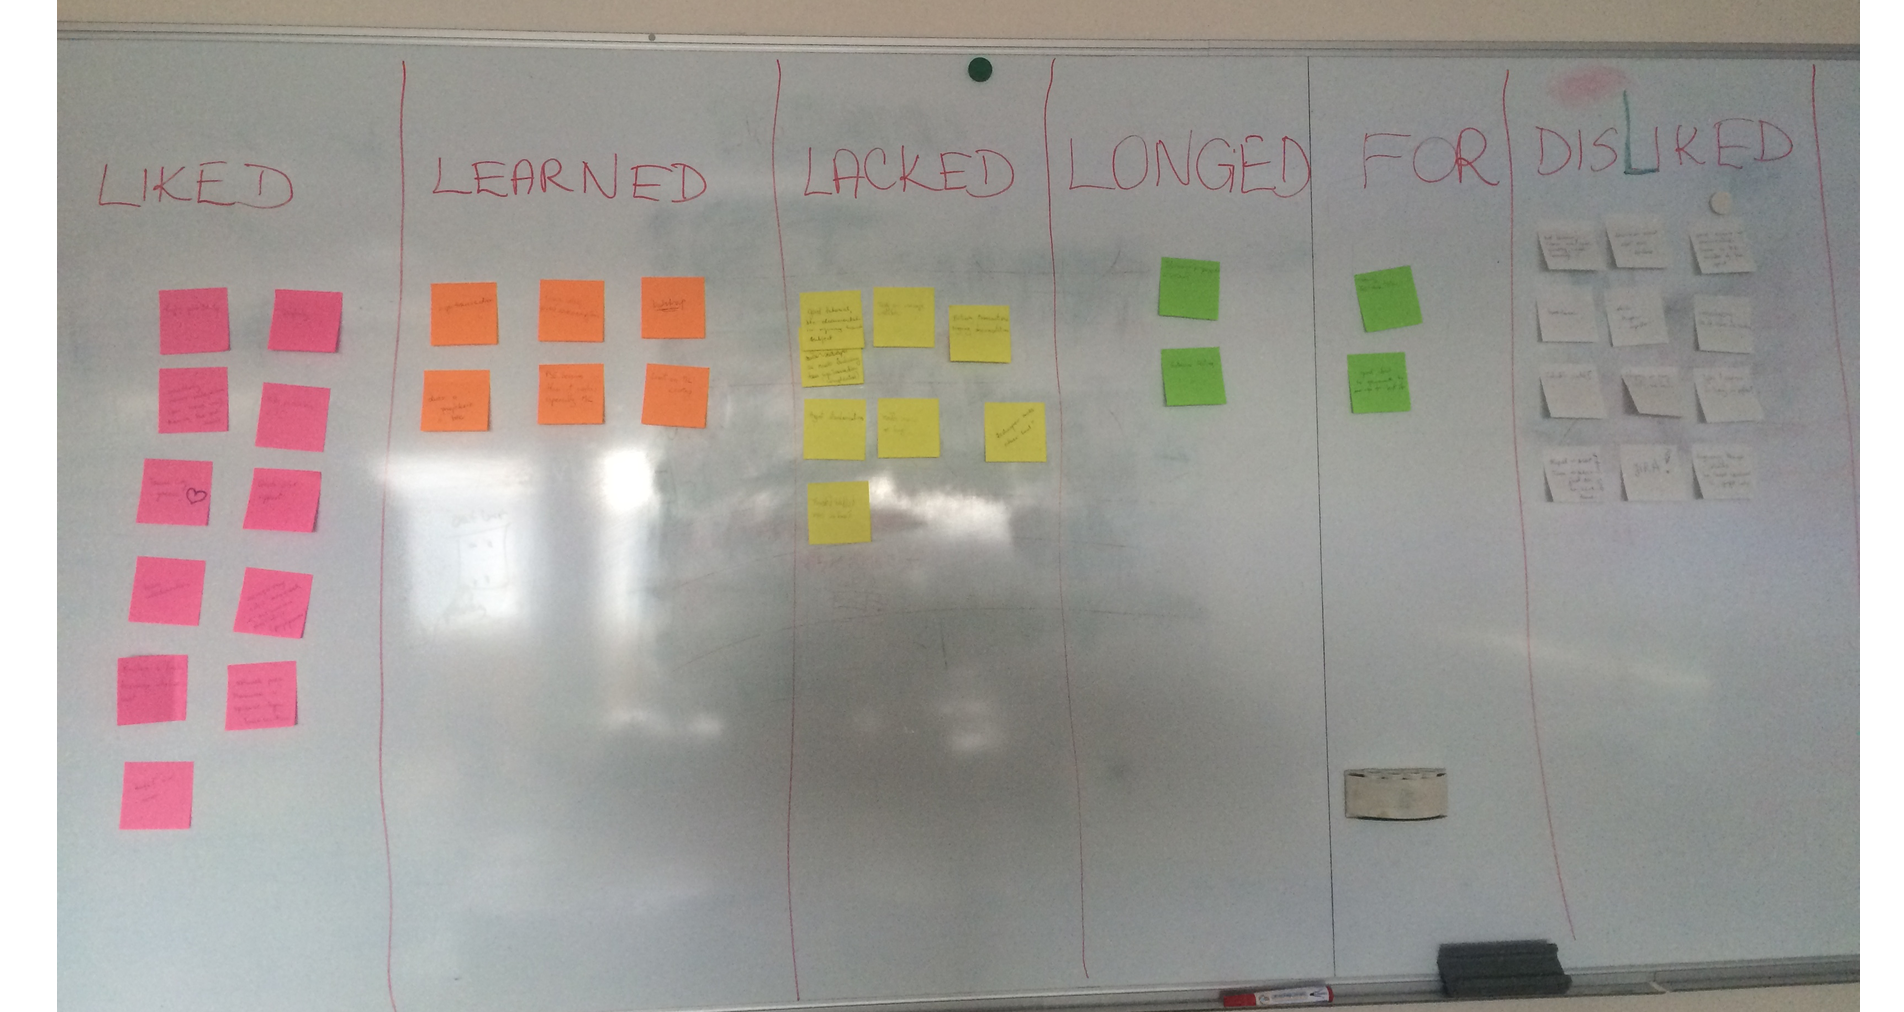
\includegraphics[width=1\textwidth]{live/5lLive2}
\end{figure}

Using the 5L's game the participants were involved in the retrospective meeting and especially using the technique with colors they even started to be competitive, who has more pink sticky-notes, or in some cases who has the most diverse pile of papers. In both teams, B and C, the game was deployed twice and was played, responsively for 50 and 65 minutes on average, as presented on \autoref{tab:groups-5LTeamResultsN}. Team B retrieved after finishing their 7th iteration 18 things they liked, 4 learned, 2 lacked, 2 longed for and 6 they loathed, and upon the 8th iteration they discovered 8 likes, 6 learns, 7 lacks, 3 things that they longed for and 8 that they loathed. In contrast, team C retrieved 15 things they liked, 4 learned, 3 lacked, 7 longed for and 10 loathing in the 24th iteration and respectively 14, 4, 2, 5 and 6 in 25th iteration. 

\begin{table}[!htbp]
	\caption{Results of the 5L's Game}
	\label{tab:groups-5LTeamResultsN}
	\begin{tabularx}{\textwidth}{|X|X|X|X|X|X|X|X|}
	\hline
		Group & Liked & Learned & Lacked & Longed for & Loathing & Time & Comment\\ \hline
		Team A &  N/A & N/A & N/A &  N/A & N/A & N/A & N/A \\ \hline
		Team B & 18 & 4 & 2 & 2 & 6 & 55 minutes & 7th iteration\\ \hline
        Team B & 8 & 6 & 7 & 3 & 8 & 45 minutes & 8th iteration\\ \hline
        Team C & 15 & 4 & 3 & 7 & 10 & 50 minutes & 24th iteration\\ \hline
        Team C & 14 & 4 & 2 & 5 & 6 & 1hour 20 minutes & 25th iteration\\ \hline
	\end{tabularx}
\end{table}

The \autoref{fig:5lResultsNew} presents the results retrieved from the participants' feedback. The results were positively surprising, because all the bars are equal or above the "Agree" statement. The participants feel the most that the involvement was increased by this technique, what is more they also agree on the fact that communication and motivation was improved by this technique and also they think this game should complement standard procedure in the retrospective meeting. The lowest result, but still very high, because exactly equal to "Agree" statement, the participants gave to the statement about whether 5L's method influence is better than using standard approach, they would also permanently implement the 5L's to the retrospective meeting, moreover they discovered increase in creativity and think that the game is easy to understand.

\begin{figure}[!htbp]
\caption{Results of deploying 5 L's game using new set of questions}
\label{fig:5lResultsNew}
\centering
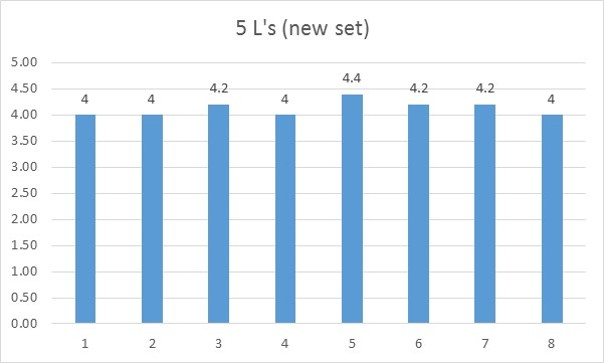
\includegraphics[width=1\textwidth]{charts/5LNewSet}
\end{figure}

\subsection{All Deployed Games Comparison}

Described in sections \nameref{sec:secondIt} games were deployed in Intel Technology Poland site in Gdańsk with collaboration with teams listed in \autoref{tab:groups-desc}. Thanks to them two games were created or improved. Moreover we were cooperating with Certified Scrum Master, Grzegorz Regliński, who also helped us in order to properly implement the games in the teams. 

\begin{figure}[!htbp]
\caption{Overall timeline of the games}
\label{fig:overallTimeline}
\centering
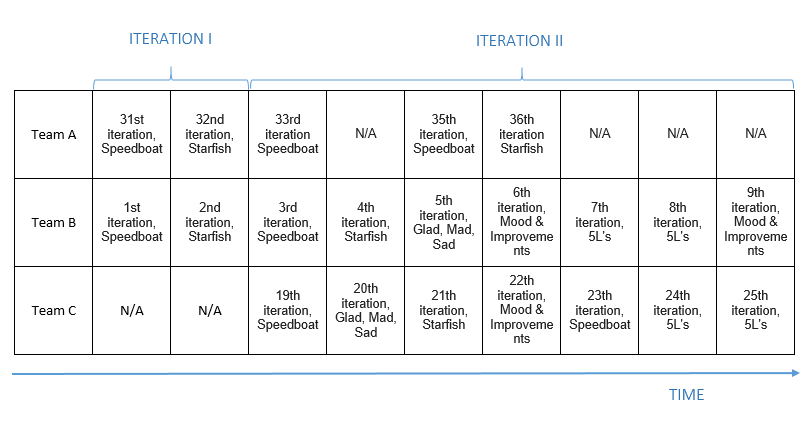
\includegraphics[width=1\textwidth]{img/overall}
\end{figure}

The overall description of deployment is presented on \autoref{fig:overallTimeline}. The figure points out, when in time the particular game were introduced, what is more in which team, while which sprint or whether it was first or second iteration of the question set.
To summarize the chart, each category responds to described games and what is more:
\begin{enumerate}
    \item The influence of this method is greater than using standard procedures.
    \begin{itemize}
        \item The participants agreed that games: Speedboat, 5L's and Starfish impacts positively on the results. \item Not as strongly, but still closer to "Agree" statement, they think that Mood and Improvements influences the outcome of retrospective comparing to standard procedures.
        \item It is hard for the members of the experiment to decide in case of Glad/Mad/Sad approach.
        \item Best games: Speedboat, 5L's and Starfish
        \item Worst game: Glad/Mad/Sad
    \end{itemize}
    \item The game should be implemented permanently instead of standard procedures.
    \begin{itemize}
        \item The participants definitely agree in case of implementing Starfish Game permanently.
        \item They have also a positive feeling in case of 5L's game in this field.
        \item The attendants of the experiment rather bow to statement "Agree" in case of Mood and Improvements.
        \item In case of Glad/Mad/Sad and Speedboat it was hard for them to decide.
        \item Best game: Starfish
        \item Worst game: Speedboat
    \end{itemize}
    \item The game might complement standard procedures.
    \begin{itemize}
        \item In case of complementing standard procedures with the introduced new approaches the Glad/Mad/Sad and 5L's had almost the same results.
        \item The result which equaled exactly "Agree" statement retrieved the Mood and Improvements approach.
        \item In case of Starfish they rather bow to "Agree" statement in case of complementing the standard procedure with the presented technique.
        \item In this category Speedboat has the worse result, it is hard for the participants to decide whether the approach should complement the standard procedures.
        \item Best game: 5L's
        \item Worst game: Speedboat
    \end{itemize}
    \item Thanks to the game the creativity of team members increased in the retrospective meeting.
    \begin{itemize}
        \item The exact value of "Agree" statement and what is more the best result in this category is assigned to 5L's technique.
        \item The game creativity in Starfish, Mood and Improvements and Glad/Mad/Sad games is also influenced, but the results are below the "Agree" statement, but heavily above the "Hard to say" opinion.
        \item The worse result was assigned to Speedboat, for the participants it was hard to determine if the influence in the creativity happened. 
        \item Best game: 5L's
        \item Worst game: Speedboat
    \end{itemize}
    \item Thanks to the game the involvement of team members increased in the retrospective meeting.
    \begin{itemize}
        \item Based on data collected from the feedback from the teams the 5L's game is the best in case of involvement of participants increment, slightly worse results performs Starfish technique.
        \item Both, Speedboat and Mood and Improvements are below "Agree" statement but significantly above the "Hard to say" opinion, so it is reasonable to claim that they likewise increasing the involvement.
        \item The Glad/Mad/Sad approach, accordingly to opinion of the team members, does not impact the involvement.
        \item Best game: 5L's
        \item Worst game: Glad/Mad/Sad
    \end{itemize}
    \item Thanks to the game the communication in the team increased in the retrospective meeting.
    \begin{itemize}
        \item The best results achieved the 5L's game in case of increasing the communication in the team.
        \item Slightly below the "Agree" statement are placed the "Mood and Improvements" and "Speedboat" games, moreover we can assume positive influence in the team communication using these approaches. 
        \item On the Starfish technique has been decided, by the attendants of the research, that it's hard to indicate whether communication has been improved.
        \item In case of Glad/Mad/Sad game it has been established that it does not have influence on the communication increase. 
        \item Best game: 5L's
        \item Worst game: Glad/Mad/Sad
    \end{itemize}
    \item Thanks to the game the motivation of team members increased in the retrospective meeting.
    \begin{itemize}
        \item The team was motivated and eager to participate especially using 5L's method. 
        \item In case of Starfish and Speedboat it has been decided that, even though the bar is slightly below the "Agree" statement, we can still establish that those methods increase teams' motivation. 
        \item For the Mood \& Improvements game, the participants determined that is hard for them to decide whether the motivation was increased using this technique.
        \item The Glad/Mad/Sad game, in case of motivating the team to be involved in the retrospective meeting, rather failed, but it is closer to the "Hard to say" statement, rather then "Disagree" opinion.
        \item Best game: 5L's
        \item Worst game: Glad/Mad/Sad
    \end{itemize}
    \item The game is easy to understand and play.
    \begin{itemize}
        \item In this category most of the games are above the "Agree" statement, which arises the conclusion that the Starfish, 5L's, Mood \& Improvements and Glad/Mad/Sad games were easy to understand by the attendants.
        \item Only one out of five approaches was for the participants hard to define whether it was easy or difficult to understand.
        \item Best game: Glad/Mad/Sad
        \item Worst game: Speedboat
    \end{itemize}
\end{enumerate}

\begin{figure}[!htbp]
\caption{Comparison of deploying all the games using new set of questions}
\label{fig:allGamesResultsNew}
\centering
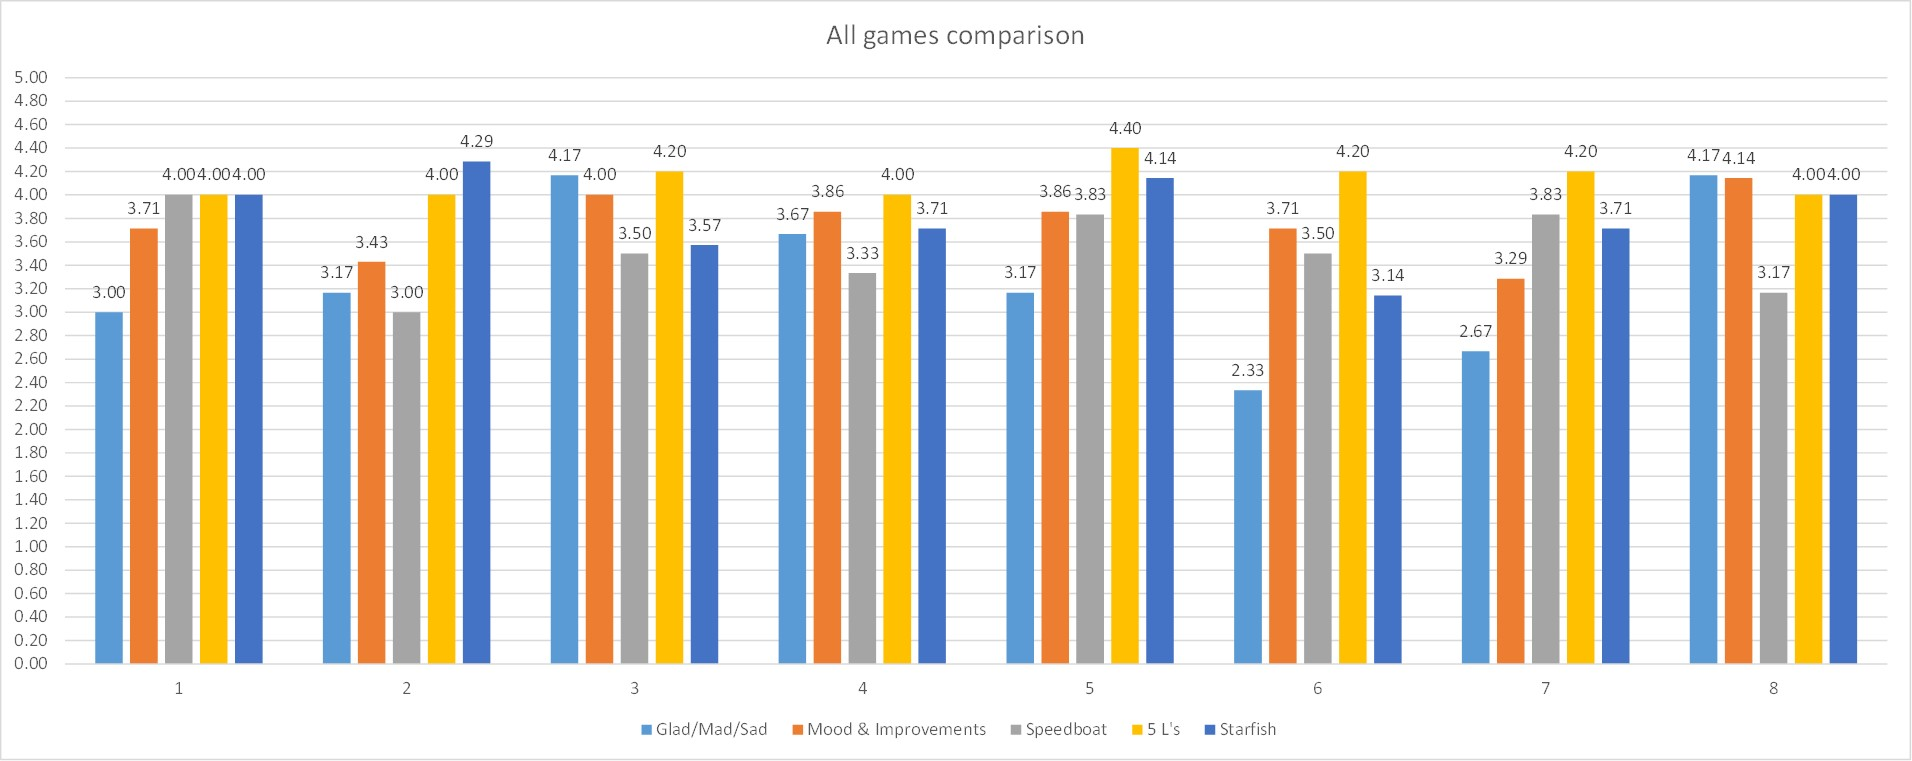
\includegraphics[width=1.1\textwidth]{charts/allGamesComp}
\end{figure}

To conclude the feedback obtained from the participants, the presented \autoref{tab:groups-overallConclusion} indicates, how many times a game transpired to be the best and the worse. In summary, the best game for all the scenarios, on the basis of attendants of the experiment opinion, is 5L's, it works well in six out of eight categories. The worse technique turn out to be the Glad/Mad/Sad, probably because of the major similarity to the standard procedures. It is not said that the Glad/Mad/Sad approach should not be used or that all the retrospective meetings should implement the 5L's method. It is advised, based on our research, to vary in case of how the retrospective meeting is being led, different techniques being deployed provides more valuable results.

\begin{table}[!htbp]
	\caption{Overall results of the games from the feedback}
	\label{tab:groups-overallConclusion}
	\begin{tabularx}{\textwidth}{|X|X|X|}
	\hline
		Game & \# of best results & \# of worse results\\ \hline
		Speedboat & 1 & 4 \\ \hline
		Starfish & 2 & None \\ \hline
        Glad/Mad/Sad & 1 & 4 \\ \hline
        5L's & 6 & None \\ \hline
        Mood \& Improvements & None & None\\ \hline
	\end{tabularx}
\end{table}

The additional \autoref{fig:groupedResults} presents a table of grouped results, green color indicates whether the threshold equal 4 or more, above "Agree" statement, was reached. The cells appointed with red color denote, where the result value was less than 3, which means "Disagree" statement. The yellow color presents results above and equal 3.5 threshold, which were also classed as "Agree" and the blue once which are above 3 and below 3.5 threshold, classified as "Hard to say" opinion. As presented in the table the 5L's game reached, as the only game, all the cells marked as above 4. The Starfish Game also retrieved almost, beside one, positive results higher than 3.5. On the other hand, the Glad/Mad/Sad is the only approach in which the less than 3 level has been obtained. In case of the other games, they perform successful outcomes in particular situation and should be used as a solution to a dedicated problem, for example for problems with the communication in the team you the Scrum Master might try the "Mood \& Improvements" approach. We can observe that the major number of results are yellow and green, which confirm the thesis, that the games increase positive factors in the retrospective meeting. The blue and the red cells are in minority. What can be also classified as a success is the fact that in the "All games together" column all the values are yellow colored, which means that in general games increase results. In the "All questions summary" column the situation is less satisfying especially for "Glad/Mad/Sad", but in the major number of games reached the threshold higher than 3.5.


\begin{figure}[!htbp]
\caption{Grouped results of all the games}
\label{fig:groupedResults}
\centering
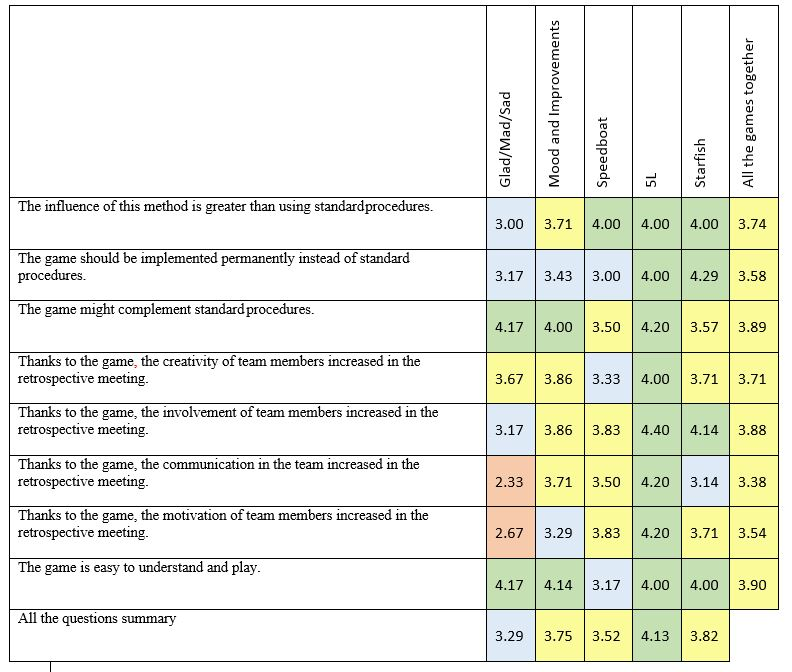
\includegraphics[width=1\textwidth]{charts/groupedResults}
\end{figure}